\documentclass [11pt]{report}						
\usepackage{fancyhdr}
\usepackage[utf8]{inputenc}
\usepackage[english]{babel}
\usepackage{gensymb}
\usepackage{amsmath,amssymb,amsfonts}
\usepackage{algorithmic}
\usepackage{graphicx}
\usepackage{textcomp}
\usepackage{xcolor}
\usepackage{siunitx}
\usepackage{indentfirst}
\usepackage[margin=2.5cm]{geometry}
\usepackage{float}
\usepackage{hyperref}
\usepackage[UKenglish]{datetime}
\usepackage{setspace}
\usepackage{hhline}

\hypersetup
{
    colorlinks=true,
    linkcolor=black,   
    urlcolor=blue,
}

\pagestyle{fancyplain}
\fancyhf{}
\fancyhead[R]{Student No. 10618407}
\fancyfoot[R]{\thepage}

\doublespacing

\begin{document}							
\title{\bf ROCO224 - Simulation of a 6DOF Robotic Arm Coursework 2020} 	
\author{Student No. 10618407} 								
\date{\today} 										
\maketitle 												
\pagenumbering{roman}						
\setcounter{page}{2}								
\tableofcontents 																	

\chapter{6DOF (6 degrees of freedom) Robotic Arm}
			
\pagenumbering{arabic}	

The 6DOF robotic arm is used throughout this project. It has six revolute joints, allowing it to have six degrees of freedom. The robot arm design is shown below, along with the subsequent coordinate frames and distances between them. These were used throughout the coursework. The 6DOF robotic arm model created in Matlab was based off this design: 


\begin{figure}[H]
\centerline{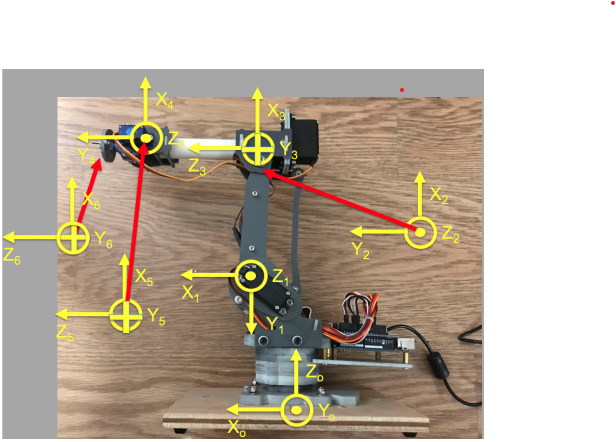
\includegraphics[width=10cm]{6DOFcoordinateframes.png}}
\caption{Coordinate frames for the 6DOF robot arm}
\label{fig}
\end{figure}

\begin{figure}[H]
\centerline{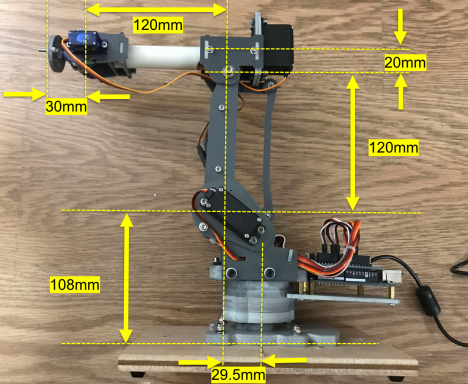
\includegraphics[width=10cm]{6DOFlengths.png}}
\caption{Distance between coordinate frames for the 6DOF robot arm}
\label{fig}
\end{figure}

\chapter{Analysis of 6DOF robotic arm}

\section{Transformation between frame \{1\}\, to frame \{0\}}

To transform between these coordinate frames, two movements are required. These are a rotation and a translation.

The rotation is 90{\degree} about the x-axis. This utilises the rotation matrix of: 
$$
\begin{bmatrix}
1&0&0\\
0&c{\theta}&-s{\theta}\\
0&s{\theta}&c{\theta}\\
\end{bmatrix}
$$

The rotational matrix of the translation between frame \{1\} and frame \{0\} is:

\begin{equation*}
\begin{matrix}
x\textsubscript{1}\\
y\textsubscript{1}\\
z\textsubscript{1}\\
\end{matrix}
= 
\begin{bmatrix}
1&0&0\\
0&0&1\\
0&-1&0\\
\end{bmatrix}
\begin{bmatrix}
x\textsubscript{0}\\
y\textsubscript{0}\\
z\textsubscript{0}\\
\end{bmatrix}
\end{equation*}

The translation between these two frames is 29.5mm in the x-axis and 108mm in the z-axis. The translation matrix for this is:

\begin{equation*}
\begin{bmatrix}
t\textsubscript{x}\\
t\textsubscript{y}\\
t\textsubscript{z}\\
\end{bmatrix}
=
\begin{bmatrix}
29.5\\
0\\
108\\
\end{bmatrix}
\end{equation*}

The rotation and translation matrices can be combined together to make a single homogeneous matrix. In Matlab these can be done both symbolically and numerically. Homogeneous equations allow both operations to be simultaneously calculated, as shown below:

\begin{figure}[H]
\centerline{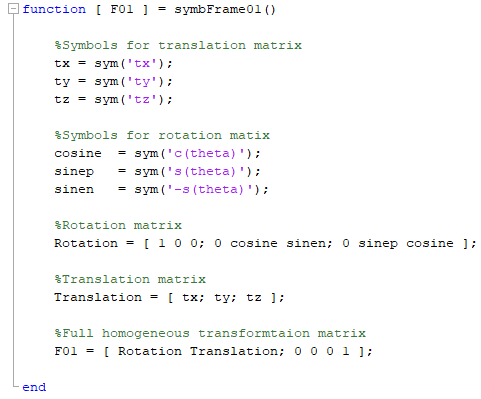
\includegraphics[width=9cm]{symbFrame01.png}}
\caption{Code for transforming between frame 1 and frame 0 symbolically in Matlab}
\label{fig}
\end{figure}

\begin{figure}[H]
\centerline{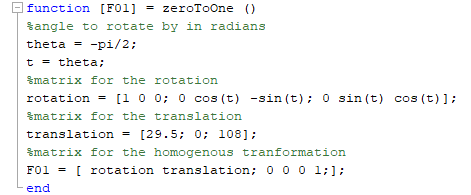
\includegraphics[width=9cm]{zeroToOnecode.png}}
\caption{Code for transforming between frame 1 and frame 0 numerically in Matlab}
\label{fig}
\end{figure}

For the transformation between frame \{1\} and frame \{0\} the homogeneous equation is as follows: 

\begin{equation*}
F01
= 
\begin{bmatrix}
1&0&0&29.5\\
0&0&1&0\\
0&-1&0&108\\
0&0&0&1\\
\end{bmatrix}
\end{equation*}

\begin{figure}[H]
\centerline{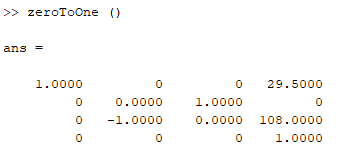
\includegraphics[width=9cm]{zeroToOneoutput.png}}
\caption{Output transformation between frame 1 and frame 0 from Matlab}
\label{fig}
\end{figure}

\section{Transformation between frame \{2\}\, to frame \{1\}}

To transform between these coordinate frames, two movements are required. These are a rotation and a translation.

The rotation is 90{\degree}about the z-axis. This utilises the rotation matrix of: 
$$
\begin{bmatrix}
c{\theta}&-s{\theta}&0\\
s{\theta}&c{\theta}&0\\
0&0&1\\
\end{bmatrix}
$$

The rotational matrix of the translation between frame \{2\} and frame \{1\} is:

\begin{equation*}
\begin{matrix}
x\textsubscript{1}\\
y\textsubscript{1}\\
z\textsubscript{1}\\
\end{matrix}
= 
\begin{bmatrix}
0&1&0\\
-1&0&0\\
0&0&1\\
\end{bmatrix}
\begin{bmatrix}
x\textsubscript{0}\\
y\textsubscript{0}\\
z\textsubscript{0}\\
\end{bmatrix}
\end{equation*}

The translation between these two frames is -120mm in the y-axis. The translation matrix for this is:

\begin{equation*}
\begin{bmatrix}
t\textsubscript{x}\\
t\textsubscript{y}\\
t\textsubscript{z}\\
\end{bmatrix}
=
\begin{bmatrix}
0\\
-120\\
0\\
\end{bmatrix}
\end{equation*}

The rotation and translation matrices can be combined together to make a single homogeneous matrix. In Matlab these can be done both symbolically and numerically. Homogeneous equations allow both operations to be simultaneously calculated, as shown below:

\begin{figure}[H]
\centerline{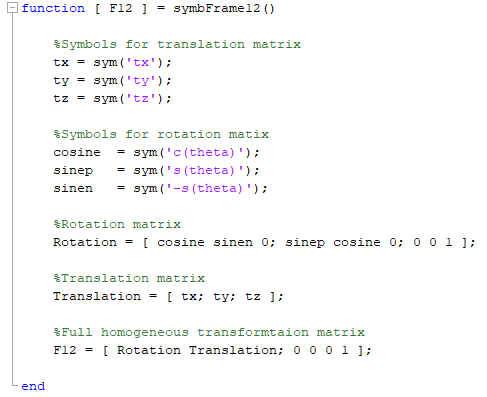
\includegraphics[width=9cm]{symbFrame12.png}}
\caption{Code for transforming between frame 2 and frame 1 symbolically in Matlab}
\label{fig}
\end{figure}

\begin{figure}[H]
\centerline{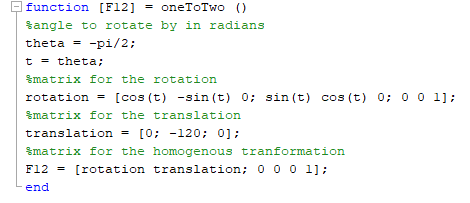
\includegraphics[width=9cm]{oneToTwocode.png}}
\caption{Code for transforming between frame 2 and frame 1 numerically in Matlab}
\label{fig}
\end{figure}

For the transformation between frame \{2\} and frame \{1\} the homogeneous equation is as follows: 

\begin{equation*}
F12
= 
\begin{bmatrix}
0&1&0&0\\
-1&0&0&-120\\
0&0&1&0\\
0&0&0&1\\
\end{bmatrix}
\end{equation*}

\begin{figure}[H]
\centerline{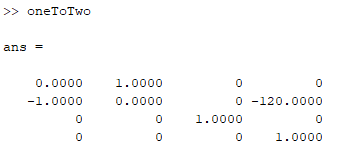
\includegraphics[width=9cm]{oneToTwooutput.png}}
\caption{Output transformation between frame 2 and frame 1 from Matlab}
\label{fig}
\end{figure}

\section{Transformation between frame \{3\}\, to frame \{2\}}

To transform between these coordinate frames, two movements are required. These are a rotation and a translation. 

The rotation is 90{\degree} about the x-axis. This utilises the rotation matrix of: 
$$
\begin{bmatrix}
1&0&0\\
0&c{\theta}&-s{\theta}\\
0&s{\theta}&c{\theta}\\
\end{bmatrix}
$$

The rotational matrix of the translation between frame \{3\} and frame \{2\} is:

\begin{equation*}
\begin{matrix}
x\textsubscript{1}\\
y\textsubscript{1}\\
z\textsubscript{1}\\
\end{matrix}
= 
\begin{bmatrix}
1&0&0\\
0&0&1\\
0&-1&0\\
\end{bmatrix}
\begin{bmatrix}
x\textsubscript{0}\\
y\textsubscript{0}\\
z\textsubscript{0}\\
\end{bmatrix}
\end{equation*}

The translation between these two frames is 20mm in the x-axis. The translation matrix for this is:

\begin{equation*}
\begin{bmatrix}
t\textsubscript{x}\\
t\textsubscript{y}\\
t\textsubscript{z}\\
\end{bmatrix}
=
\begin{bmatrix}
20\\
0\\
0\\
\end{bmatrix}
\end{equation*}

The rotation and translation matrices can be combined together to make a single homogeneous matrix. In Matlab these can be done both symbolically and numerically. Homogeneous equations allow both operations to be simultaneously calculated, as shown below:

\begin{figure}[H]
\centerline{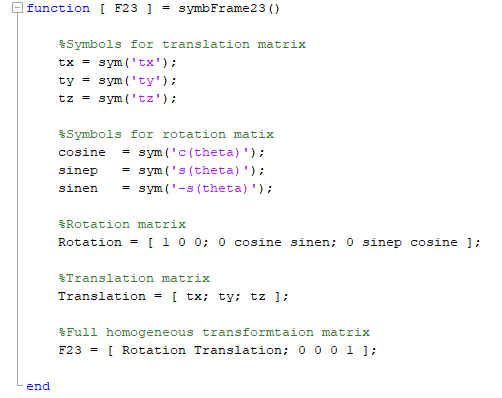
\includegraphics[width=9cm]{symbFrame23.png}}
\caption{Code for transforming between frame 3 and frame 2 symbolically in Matlab}
\label{fig}
\end{figure}

\begin{figure}[H]
\centerline{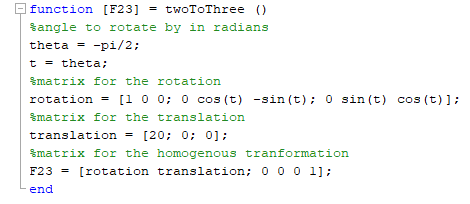
\includegraphics[width=9cm]{twoToThreecode.png}}
\caption{Code for transforming between frame 3 and frame 2 numerically in Matlab}
\label{fig}
\end{figure}

For the transformation between frame \{3\} and frame \{2\} the homogeneous equation is as follows: 

\begin{equation*}
F23
= 
\begin{bmatrix}
1&0&0&20\\
0&0&1&0\\
0&-1&0&0\\
0&0&0&1\\
\end{bmatrix}
\end{equation*}

\begin{figure}[H]
\centerline{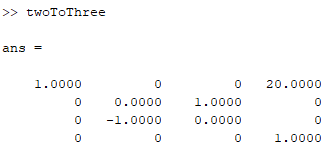
\includegraphics[width=9cm]{twoToThreeoutput.png}}
\caption{Output transformation between frame 3 and frame 2 from Matlab}
\label{fig}
\end{figure}

\section{Transformation between frame \{4\}\, to frame \{3\}}

To transform between these coordinate frames, two movements are required. Thse are a rotation and a translation. 

The rotation is 90{\degree} about the x-axis. This utilises the rotation matrix of: 
$$
\begin{bmatrix}
1&0&0\\
0&c{\theta}&s{\theta}\\
0&-s{\theta}&c{\theta}\\
\end{bmatrix}
$$

The rotational matrix of the translation between frame \{4\} and frame \{3\} is:

\begin{equation*}
\begin{matrix}
x\textsubscript{1}\\
y\textsubscript{1}\\
z\textsubscript{1}\\
\end{matrix}
= 
\begin{bmatrix}
1&0&0\\
0&0&1\\
0&-1&0\\
\end{bmatrix}
\begin{bmatrix}
x\textsubscript{0}\\
y\textsubscript{0}\\
z\textsubscript{0}\\
\end{bmatrix}
\end{equation*}

The translation between these two frames is 120mm in the z-axis. The translation matrix for this is:

\begin{equation*}
\begin{bmatrix}
t\textsubscript{x}\\
t\textsubscript{y}\\
t\textsubscript{z}\\
\end{bmatrix}
=
\begin{bmatrix}
0\\
0\\
120\\
\end{bmatrix}
\end{equation*}

The rotation and translation matrices can be combined together to make a single homogeneous matrix. In Matlab these can be done both symbolically and numerically. Homogeneous equations allow both operations to be simultaneously calculated, as shown below:

\begin{figure}[H]
\centerline{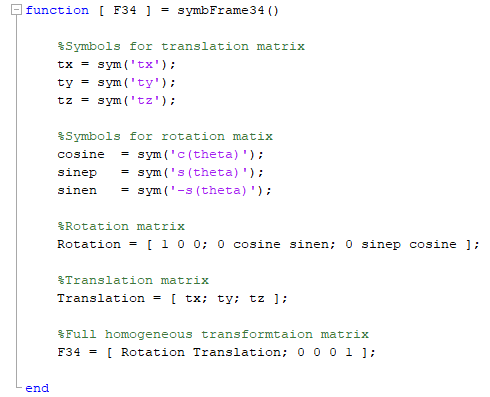
\includegraphics[width=9cm]{symbFrame34.png}}
\caption{Code for transforming between frame 4 and frame 3 symbolically in Matlab}
\label{fig}
\end{figure}


\begin{figure}[H]
\centerline{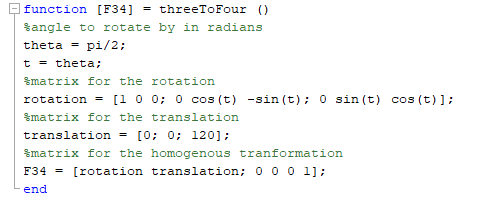
\includegraphics[width=9cm]{threeToFourcode.png}}
\caption{Code for transforming between frame 4 and frame 3 numerically in Matlab}
\label{fig}
\end{figure}

For the transformation between frame \{4\} and frame \{3\} the homogeneous equation is as follows: 

\begin{equation*}
F34
= 
\begin{bmatrix}
1&0&0&0\\
0&0&-1&0\\
0&1&0&120\\
0&0&0&1\\
\end{bmatrix}
\end{equation*}

\begin{figure}[H]
\centerline{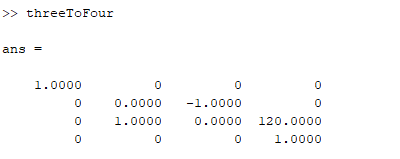
\includegraphics[width=9cm]{threeToFouroutput.png}}
\caption{Output transformation between frame 4 and frame 3 from Matlab}
\label{fig}
\end{figure}

\section{Transformation between frame \{5\}\, to frame \{4\}}

To transform between these coordinate frames, two movements are required. These are a rotation and a translation. 

The rotation is 90{\degree} about the x-axis. This utilises the rotation matrix of: 
$$
\begin{bmatrix}
1&0&0\\
0&c{\theta}&s{\theta}\\
0&-s{\theta}&c{\theta}\\
\end{bmatrix}
$$

The rotational matrix of the translation between frame \{5\} and frame \{4\} is:

\begin{equation*}
\begin{matrix}
x\textsubscript{1}\\
y\textsubscript{1}\\
z\textsubscript{1}\\
\end{matrix}
= 
\begin{bmatrix}
1&0&0\\
0&0&1\\
0&-1&0\\
\end{bmatrix}
\begin{bmatrix}
x\textsubscript{0}\\
y\textsubscript{0}\\
z\textsubscript{0}\\
\end{bmatrix}
\end{equation*}

For the transformation between frame 5 and frame 4 there is no translation between the two coordinate frames, therefore the translation matrix is equal to 0. 

\begin{equation*}
\begin{bmatrix}
t\textsubscript{x}\\
t\textsubscript{y}\\
t\textsubscript{z}\\
\end{bmatrix}
=
\begin{bmatrix}
0\\
0\\
0\\
\end{bmatrix}
\end{equation*}

The rotation and translation matrices can be combined together to make a single homogeneous matrix. In Matlab these can be done both symbolically and numerically. Homogeneous equations allow both operations to be simultaneously calculated, as shown below:

\begin{figure}[H]
\centerline{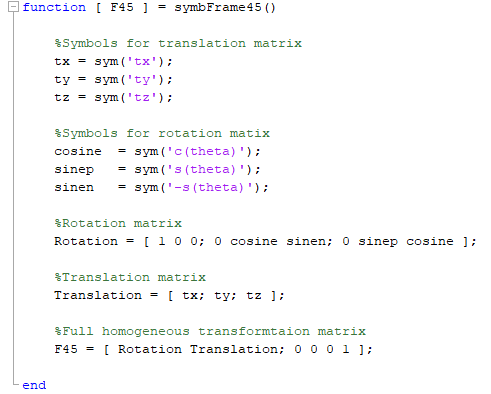
\includegraphics[width=9cm]{symbFrame45.png}}
\caption{Code for transforming between frame 5 and frame 4 symbolically in Matlab}
\label{fig}
\end{figure}


\begin{figure}[H]
\centerline{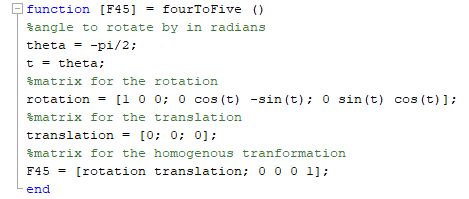
\includegraphics[width=9cm]{fourToFivecode.png}}
\caption{Code for transforming between frame 5 and frame 4 numerically in Matlab}
\label{fig}
\end{figure}

For the transformation between frame \{5\} and frame \{4\} the homogeneous equation is as follows: 

\begin{equation*}
F45
= 
\begin{bmatrix}
1&0&0&0\\
0&0&1&0\\
0&-1&0&0\\
0&0&0&1\\
\end{bmatrix}
\end{equation*}

\begin{figure}[H]
\centerline{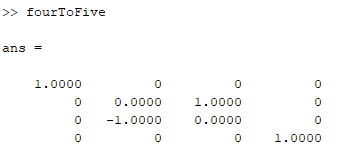
\includegraphics[width=9cm]{fourToFiveoutput.png}}
\caption{Output transformation between frame 5 and frame 4 from Matlab}
\label{fig}
\end{figure}

\section{Transformation between frame \{6\}\, to frame \{5\}}

To transform between these coordinate frames, two movements are required. These are a rotation and a translation. 

There is no rotation between the two coordinate frames for this transformation. Because of this, an identity matrix is used: 
$$
\begin{bmatrix}
1&0&0\\
0&1&0\\
0&0&1\\
\end{bmatrix}
$$

The rotational matrix of the translation between frame \{6\} and frame \{5\} is:

\begin{equation*}
\begin{matrix}
x\textsubscript{1}\\
y\textsubscript{1}\\
z\textsubscript{1}\\
\end{matrix}
= 
\begin{bmatrix}
1&0&0\\
0&1&0\\
0&0&1\\
\end{bmatrix}
\begin{bmatrix}
x\textsubscript{0}\\
y\textsubscript{0}\\
z\textsubscript{0}\\
\end{bmatrix}
\end{equation*}

The translation between these two frames is 30mm in the z-axis. The translation matrix for this is:

\begin{equation*}
\begin{bmatrix}
t\textsubscript{x}\\
t\textsubscript{y}\\
t\textsubscript{z}\\
\end{bmatrix}
=
\begin{bmatrix}
0\\
0\\
30\\
\end{bmatrix}
\end{equation*}

The rotation and translation matrices can be combined together to make a single homogeneous matrix. In Matlab these can be done both symbolically and numerically. Homogeneous equations allow both operations to be simultaneously calculated, as shown below:

\begin{figure}[H]
\centerline{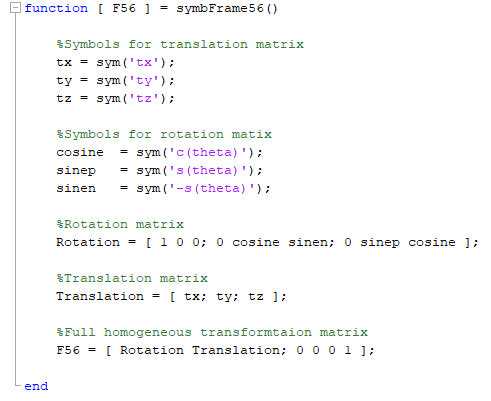
\includegraphics[width=9cm]{symbFrame56.png}}
\caption{Code for transforming between frame 6 and frame 5 symbolically in Matlab}
\label{fig}
\end{figure}


\begin{figure}[H]
\centerline{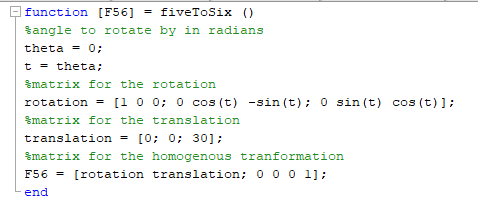
\includegraphics[width=9cm]{fiveToSixcode.png}}
\caption{Code for transforming between frame 6 and frame 5 symbolically in Matlab}
\label{fig}
\end{figure}

For the transformation between frame \{6\} and frame \{5\} the homogeneous equation is as follows: 

\begin{equation*}
F56
= 
\begin{bmatrix}
1&0&0&0\\
0&1&0&0\\
0&0&1&30\\
0&0&0&1\\
\end{bmatrix}
\end{equation*}

\begin{figure}[H]
\centerline{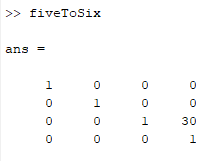
\includegraphics[width=9cm]{fiveToSixoutput.png}}
\caption{Output transformation between frame 6 and frame 5 in Matlab}
\label{fig}
\end{figure}

\section{Forward kinematics: frame \{6\}\, to frame \{0\}}

To get from frame \{6\} to frame \{0\}, you need to multiply together the homogeneous matrices of the coordinate frames already calculated. 

\begin{equation*}
F06
=
\begin{bmatrix}
0 & 0 & 1 & 179.5\\
0 & -1 & 0 & 0\\
1 & 0 & 0 & 248\\
0 & 0 & 0 & 1\\
\end{bmatrix}
\end{equation*}

\begin{figure}[H]
\centerline{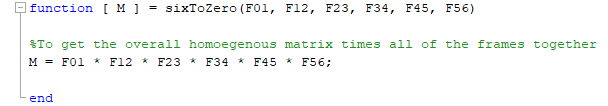
\includegraphics[width=10cm]{zeroToSixcode.png}}
\caption{Output transformation between frame 6 and frame 0 in Matlab}
\label{fig}
\end{figure}
The matrix below is the homogeneous transformation matrix for the transformation between the frames \{0\} and \{6\}: 

\begin{figure}[H]
\centerline{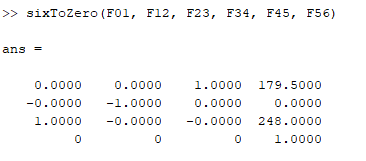
\includegraphics[width=8cm]{sixToZeroOutput.png}}
\caption{Output transformation between frame 6 and frame 0 in Matlab}
\label{fig}
\end{figure}

\chapter{Analysis of 6DOF arm using classical Denavit-Hartenberg Parameters}

\section{Build the Denavit-Hartenberg table}
\subsection{What is Denavit-Hartenberg?}

In mechanics, the Denavit-Hartenberg (DH) parameters are one convention for attaching links of a robot manipulator to a reference frame. Coordinate frames are attached to the joints between links using a transformation in reference to both [X] and [Z]. These can be used for every joint of a robot consisting of n links. 

\begin{equation*}
[T] = [Z\textsubscript{1}][X\textsubscript{1}][Z\textsubscript{2}][X\textsubscript{2}]...[Z\textsubscript{n-1}][X\textsubscript{n-1}][Z\textsubscript{n}][X\textsubscript{n}]
\end{equation*}

These reference frames are laid out in the following way:
\begin{enumerate}
\item z-axis: direction of the joint
\item x-axis: parallel to the common normal
\item y-axis: follows the right hand rule and is dictated by the z-axis and the x-axis
\end{enumerate}

\subsection{Denavit-Hartenberg Table}

The Denavit-Hartenberg table, for the 6DOF robotic arm used in this coursework, is shown below:

\begin{center}
\begin{tabular}{ ||c||c|c|c|c|| } 
 \hline
 & $\theta$ & $\alpha$ & a & d \\ 
\hhline{#=#=|=|=|=#}
 1 & 0 & -$\pi$/2 & 29.5 & 108\\
\hline 
 2 & -$\pi$/2 & 0 & 120 &0\\ 
\hline 
 3 & 0 & -$\pi$/2 & 20 &0\\ 
\hline 
 4 & 0 & $\pi$/2 & 0 & 120\\ 
\hline 
 5 & 0 & -$\pi$/2 & 0 & 0\\ 
\hline 
 6 & 0 & 0 & 0 & 30\\ 
\hline
\end{tabular}
\end{center}

Where:
\begin{itemize}
\item $\theta$ is the angle around the previous z-axis, from the old x to the new x
\item $\alpha$ is the angle around the common normal, from the old z to the new z
\item a is the length of the common normal
\item d is the offset along the previous z-axis
\end{itemize}

\section{Forward kinematics}

The following code is used to setup both a Denavit-Hartenberg table in Matlab and an environment for the robotic arm to be displayed. The Denavit-Hartenberg table creates all the serial links for the robotic arm. The mid values ($\theta$) of 0 set the robotic arm to its default position.

\begin{figure}[H]
\centerline{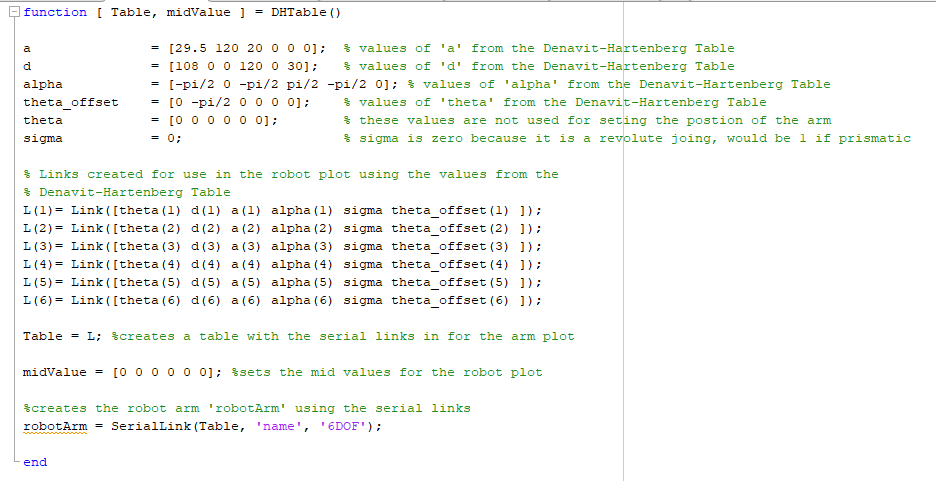
\includegraphics[width=12cm]{DHTablewithoutplot.png}}
\caption{Code to setup the Denavit-Hartenberg table and the robotic arm}
\label{fig}
\end{figure}

\begin{figure}[H]
\centerline{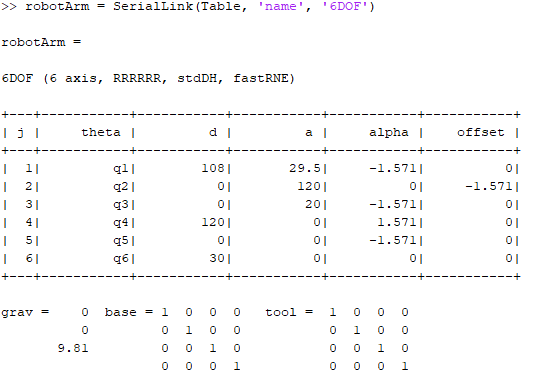
\includegraphics[width=12cm]{robotArmDHTable.png}}
\caption{Output Denavit-Hartenberg table for the robot arm in Matlab}
\label{fig}
\end{figure}

\section{Display default configuration}

The code below is used to create a static model of the 6DOF robotic arm. It utilises the serial links created using the Denavit-Hartenberg table. The robot arm is in its `natural' position (with mid values equal to zero). The robot arm is plotted in a work space that is 1000x1000x600. This allows the robot to extend its full range of movements without going outside the bounds of the work space. 

\begin{figure}[H]
\centerline{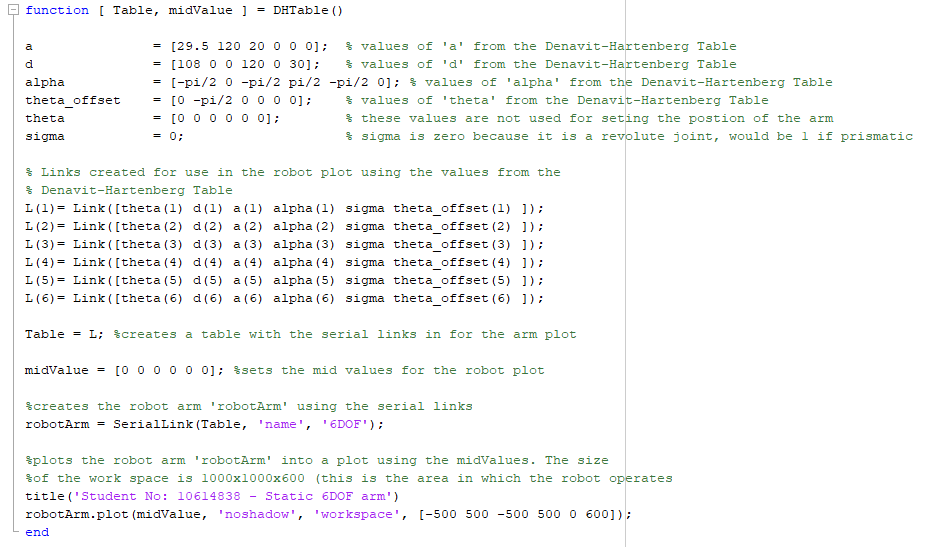
\includegraphics[width=12cm]{StaticRoboticArmCode.png}}
\caption{Code to setup and plot the robotic arm}
\label{fig}
\end{figure}

\begin{figure}[H]
\centerline{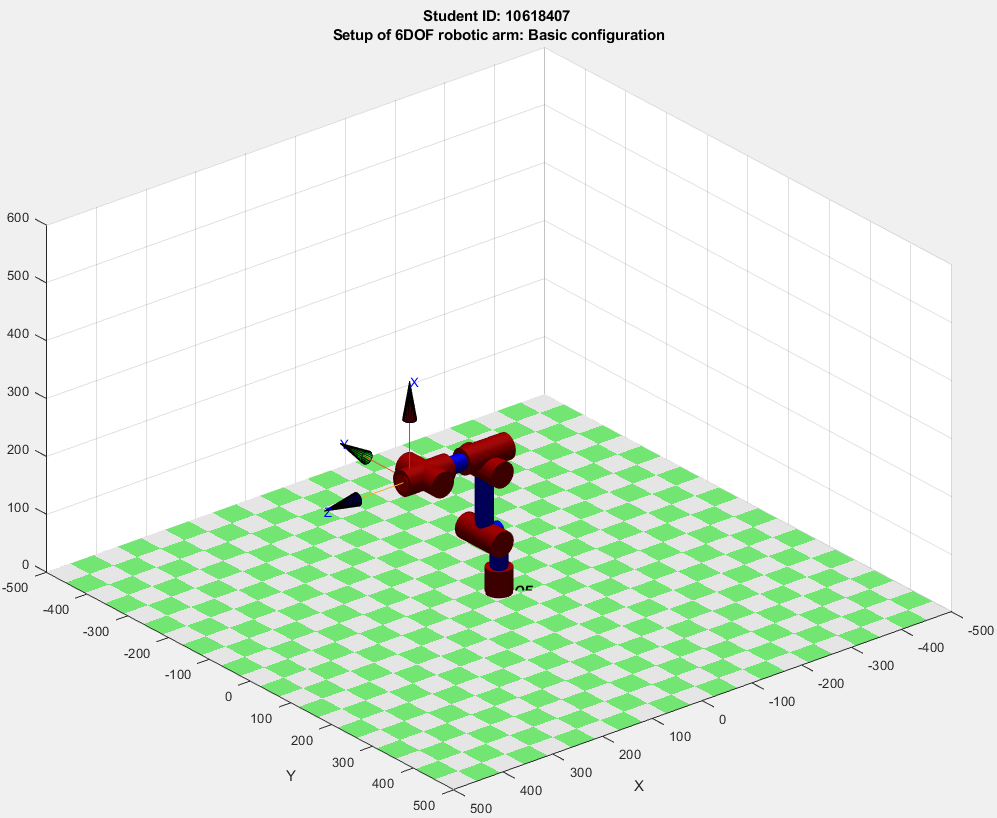
\includegraphics[width=12cm]{StaticRoboticArm.png}}
\caption{Setup of 6DOF robotic arm: Basic (natural) configuration}
\label{fig}
\end{figure}

\newpage
\section{Build interactive model}

The interactive mode allows the robot's joints to be manipulated using various sliders along the left hand side of the work space. This allows the range of the robot's movement to be analysed in conjunction with one another.

\begin{figure}[H]
\centerline{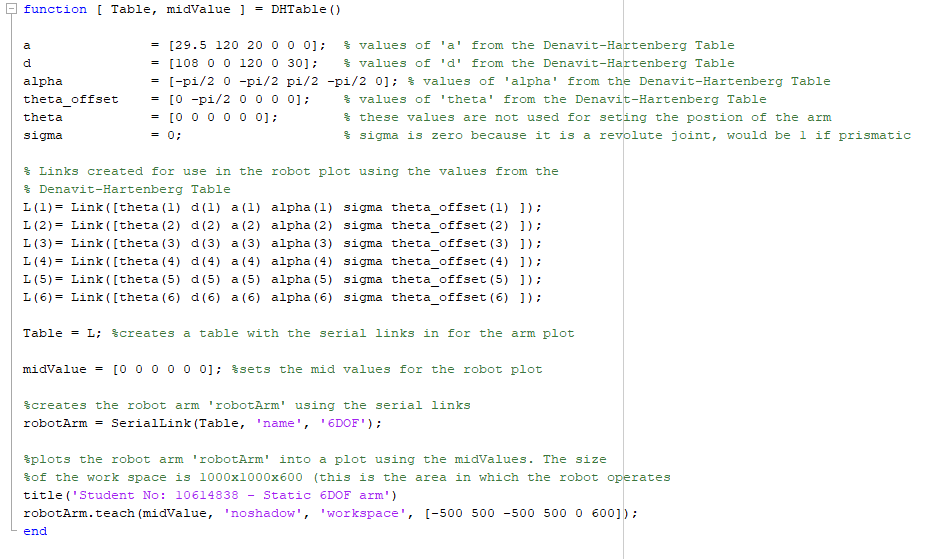
\includegraphics[width=14cm]{teachRobotArmCode.png}}
\caption{Code to setup and plot the robotic arm in teach mode}
\label{fig}
\end{figure}

\begin{figure}[H]
\centerline{\includegraphics[width=18cm]{teachRobotArmPlot.png}}
\caption{Robotic arm in teach mode}
\label{fig}
\end{figure}

To see the teach mode working in a video use the following link: \href{https://youtu.be/RaQ-lbTKuEQ}{https://youtu.be/RaQ-lbTKuEQ}.

\section{Build a scatter plot of random arm locations}

Building a scatter plot of random arm locations allows the evaluation of the positions the robot can be maneuvered into, along with its reach. The following code shows how the random points of the robotic arm were acquired and plotted onto the preexisting model. In total there are 10,000 random points plotted in the figure.

\begin{figure}[H]
\centerline{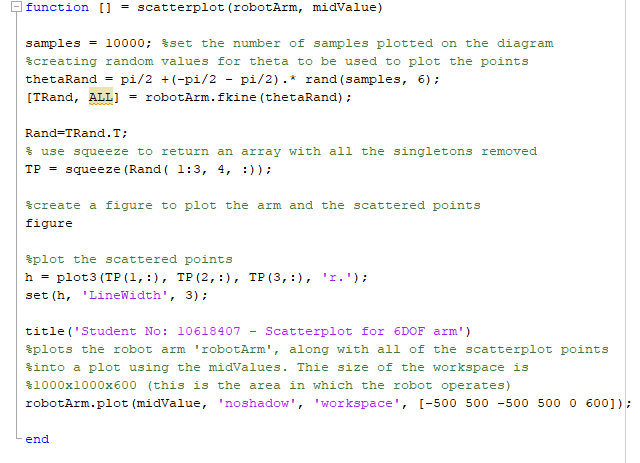
\includegraphics[width=12cm]{scatterplotCode.png}}
\caption{Code for plotting the scattered points in Matlab}
\label{fig}
\end{figure}

Below are two views of the scattered points overlaid on the static arm configuration. These show the range of motion that the robot arm can theoretically achieve:


\begin{figure}[H]
\centerline{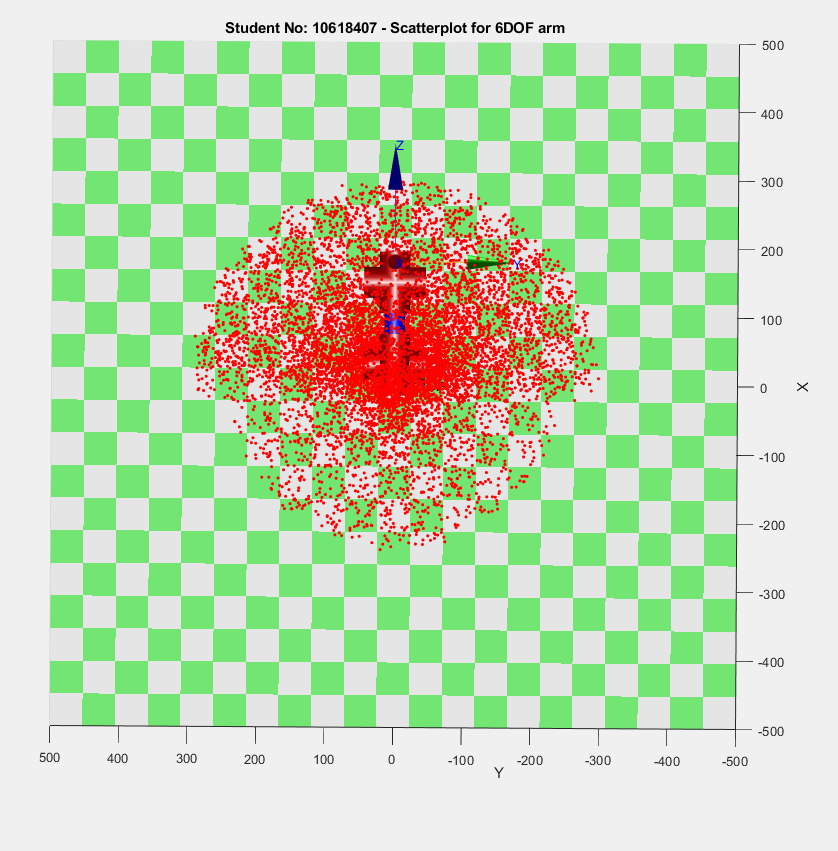
\includegraphics[width=10cm]{StaticRoboticArmwithScatteredPointsTopView.png}}
\caption{Static robotic arm with scattered points (top view)}
\label{fig}
\end{figure}

\begin{figure}[H]
\centerline{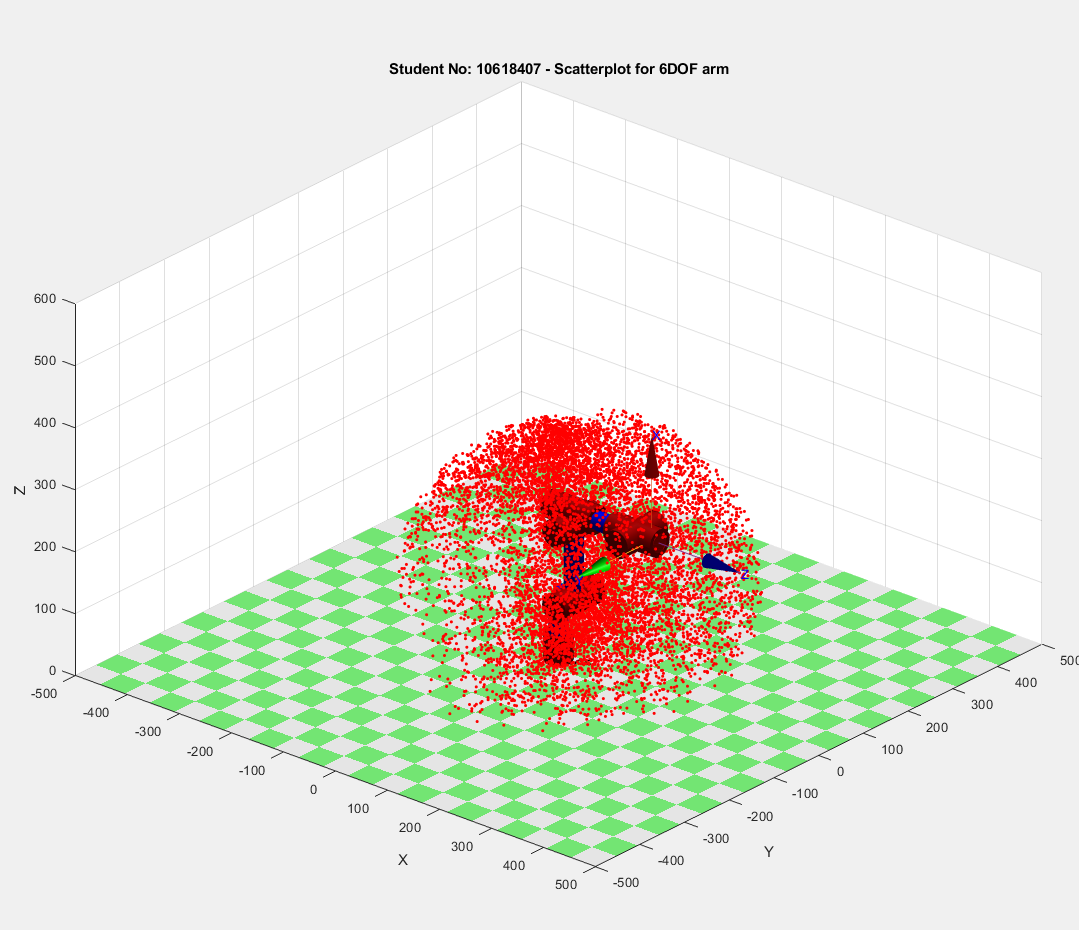
\includegraphics[width=10cm]{StaticRoboticArmwithScatteredPointsIsometricView.png}}
\caption{Static robotic arm with scattered points (isometric view)}
\label{fig}
\end{figure}  

\section{Animated trajectory following}

Animated trajectory following allows you to see how the joints of the robot move when the end effector is moving between given points inside its reach. The code below sets up the points for the robot arm to move between, along with the computation allowing the robot arm's end effector to follow the trajectory. The arm interpolates data between these points allowing it to move in the shortest path possible. All of these positions are put into a matrix and plotted using the robot arm.

\begin{figure}[H]
\centerline{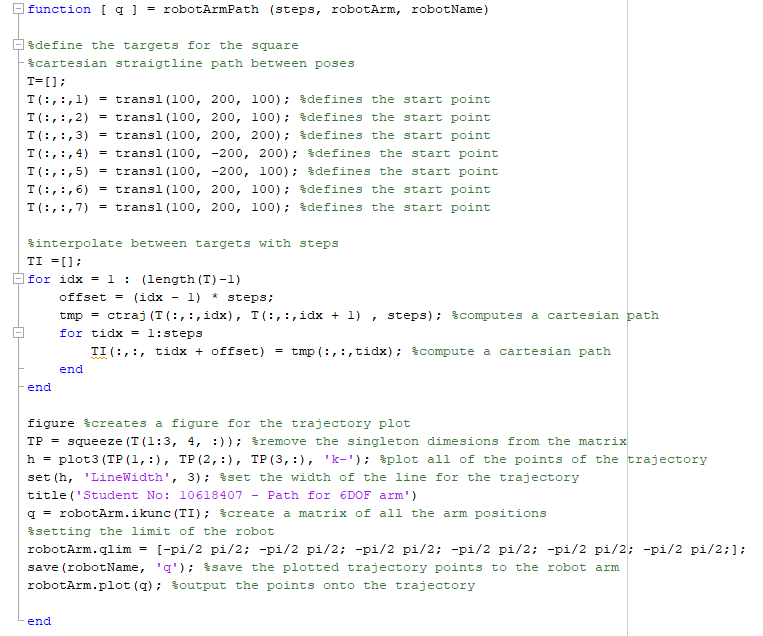
\includegraphics[width=10cm]{robotArmPathCode.png}}
\caption{Code for plotting the path for the robot arm to follow}
\label{fig}
\end{figure} 

Below is a static view of the robot arm and its path of travel: 

\begin{figure}[H]
\centerline{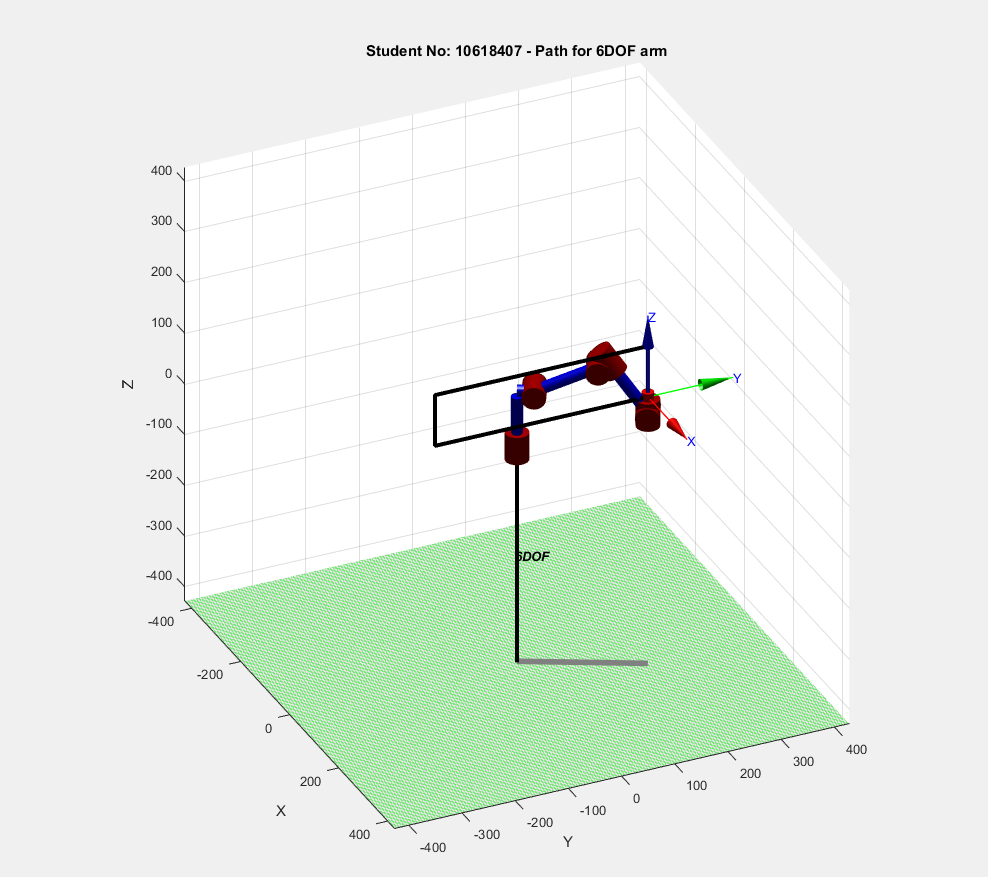
\includegraphics[width=14cm]{movingRobotArm.png}}
\caption{Static robotic arm with movement path}
\label{fig}
\end{figure} 

To see the robot arm following the path in a video use the following link: \href{https://youtu.be/U7mfT64HJG0}{https://youtu.be/U7mfT64HJG0}\\

As the end effector moves across a linear path, the joint angles change. The joint angles do not move linearly like the end effector. This is due to the nature of the movement of the robot. Because of this, it is important to be able to evaluate how the joint angles move with the end effector. This is used heavily in robotics to judge how an end effector or joints will move. This is shown in the graph below along with the code to produce to trajectory plot graph:

\begin{figure}[H]
\centerline{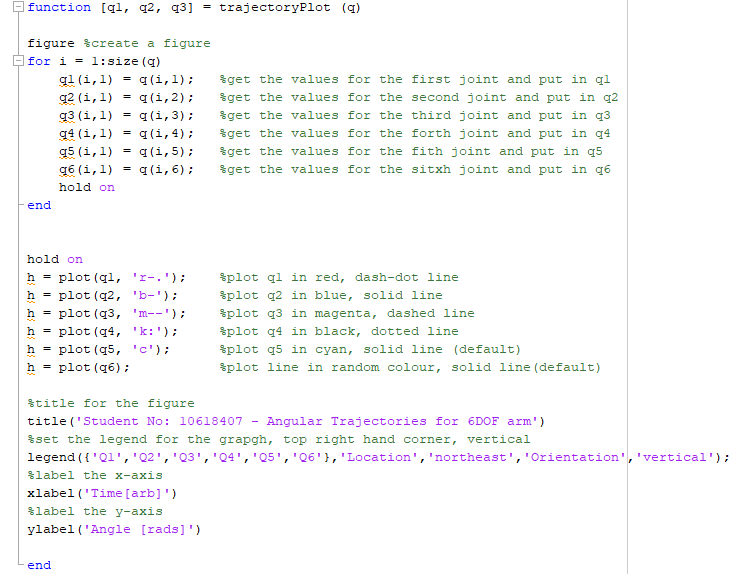
\includegraphics[width=12cm]{trajectoryPlotCode.png}}
\caption{Matlab code to produce the trajectory plot graph}
\label{fig}
\end{figure} 

\begin{figure}[H]
\centerline{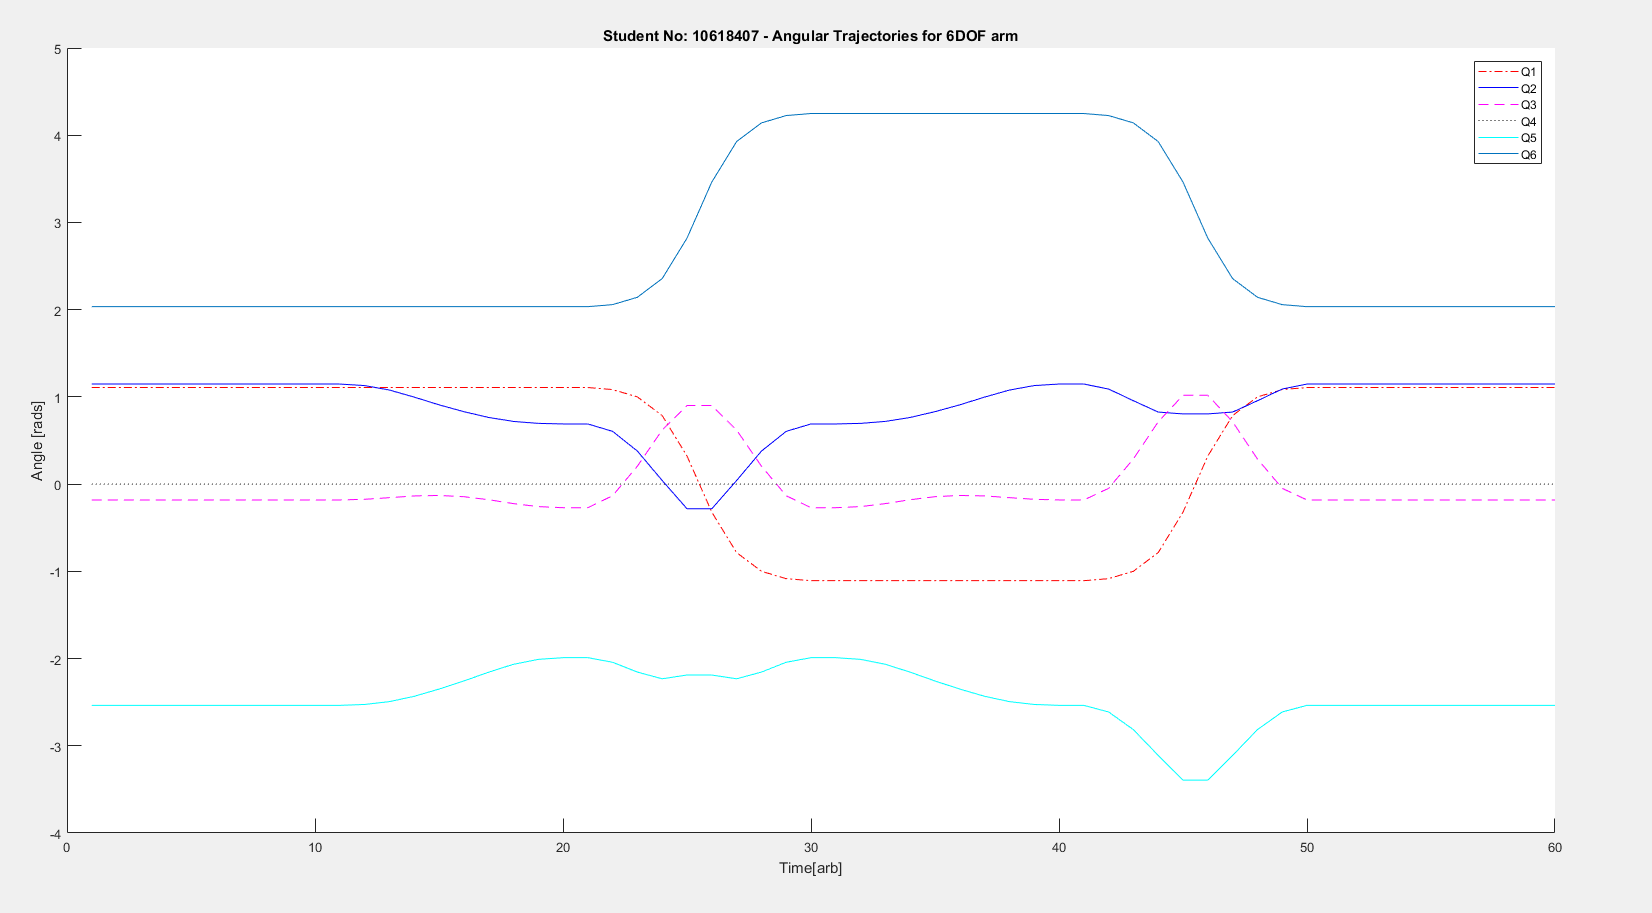
\includegraphics[width=20cm]{trajectoryPlot.png}}
\caption{Angular trajectory of robot arm joints }
\label{fig}
\end{figure} 


\end{document}
 
 

 

